% You should title the file with a .tex extension (hw1.tex, for example)
\documentclass[11pt]{article}

\usepackage{hyperref}
\usepackage{amsmath}
\usepackage{mathtools}
\usepackage{amssymb}
\usepackage{wrapfig}
\usepackage{fancyhdr}
\usepackage{tikz-qtree}
\usepackage{tikz-qtree-compat}
\usepackage[normalem]{ulem}
\usepackage{tikz}
\usepackage{graphicx}
\DeclareMathOperator*{\argmin}{argmin}
\DeclareMathOperator*{\argmax}{argmax}

\oddsidemargin0cm
\topmargin-2cm     %I recommend adding these three lines to increase the 
\textwidth16.5cm   %amount of usable space on the page (and save trees)
\textheight23.5cm  

\newcommand{\question}[2] {\vspace{.25in} \hrule\vspace{0.5em}
\noindent{\bf #1: #2} \vspace{0.5em}
\hrule \vspace{.10in}}
\renewcommand{\part}[1] {\vspace{.10in} {\bf (#1)}}

\newcommand{\myname}{Sean Bittner}
\newcommand{\myandrew}{srb2201@columbia.edu}
\newcommand{\myhwnum}{12}

\setlength{\parindent}{0pt}
\setlength{\parskip}{5pt plus 1pt}
 
\DeclarePairedDelimiter\abs{\lvert}{\rvert}%
 %
\pagestyle{fancyplain}
\rhead{\fancyplain{}{\myname\\ \myandrew}}

\begin{document}

\medskip                        % Skip a "medium" amount of space
                                % (latex determines what medium is)
                                % Also try: \bigskip, \littleskip

\thispagestyle{plain}
\begin{center}                  % Center the following lines
{\Large Input/output properties of neuron-type population model of V1} \\
Sean Bittner \\
May 12, 2020 \\
\end{center}

\section{Introduction}
In section 3.3 of our bioRxiv preprint \cite{bittner2019interrogating}, we analyze the input/output properties of a 4 neuron-type model of V1.  
We identify degeneracies and sensitivities of neuron-type responses w.r.t specific inputs by visual inspection of the EPI distributions.  
In my opinion, these ``novel insights" are not particularly interesting.
Furthermore, these insights are easily obtained using an existing method -- approximate Bayesian computation (ABC).  

In this write-up, I present a new line of inquiry in the same V1 circuit model as the paper.
Rather than conditioning on levels of increase of each neuron-type, we condition on the stabilization of each neuron-type.
EPI then presents us with a distribution of stimulation to this V1 circuit that does not change much a particular neuron-type response.

First, I show EPI converges to a distribution covering the set of samples produced by ABC.
This important sanity check, along with some ABC bias visualization, will make nice appendix figures.
Then, I show how EPI readily identifies the most efficacious patterns of stimulation.
Finally, we confirm two distinct mechanisms of E-population stabilization using EPI on the V1 model with inactivated populations.

\section{V1 model (same as bioRxiv post)}
We consider a four-dimensional circuit model with dynamical state given by the firing rate $x$ of each neuron-type population $x = \left[x_E, x_P , x_S, x_V \right]^\top$ (Fig. 1A). 
Given a time constant of $\tau = 20$ ms and a power $n = 2$, the dynamics are driven by the rectified and exponentiated sum of recurrent ($Wx$) and external $h$ inputs:

\begin{equation}
\tau \frac{dx}{dt} = -x + [W x+ h]_+^n.
\end{equation}

\begin{center}
\textbf{Figure 1: V1 model} \\
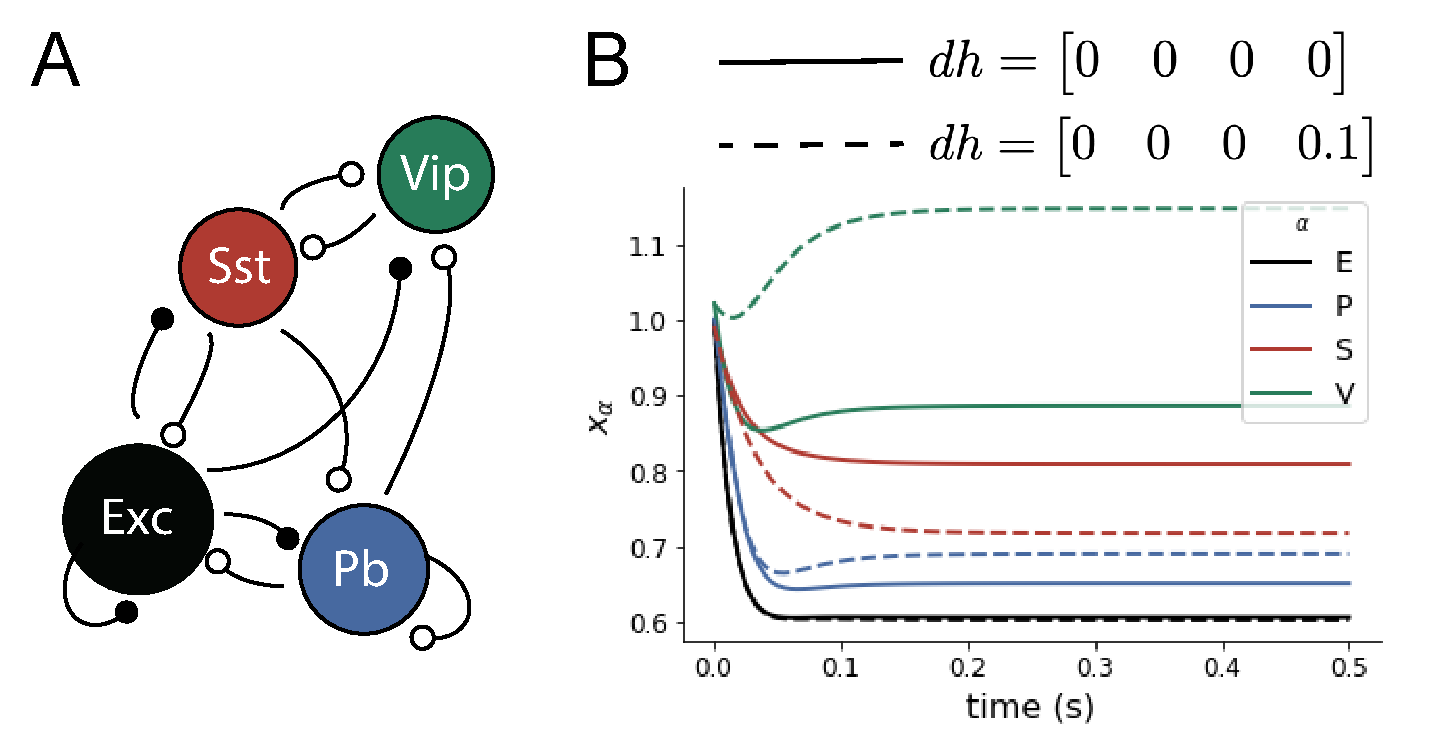
\includegraphics[scale=.4]{figs/V1_responses.pdf}
\end{center}

We considered fixed effective connectivity weights $W$ approximated from experimental recordings of publicly available datasets of mouse V1 \cite{allen2018layer, billeh2019systematic}.
The input $h = b + dh$ is comprised of a baseline input  $b = \left[ b_E, b_P , b_S , b_V \right]^\top = \left[ 1, 1, 1 ,1.25 \right]^\top$  and a differential input $dh = \left[ dh_E , dh_P , dh_S , dh_V\right]^\top$ to each neuron-type population.  

We want to know the differential inputs $dh$ that maintain the steady state $x_{\alpha}$ for $\alpha \in \{E, P, S, V\}$. 
We see from Figure 1B that input to a single population in the recurrent circuit elicits a variety of responses across populations: E same, P up, S down, and V up.
We define the differential steady state $dx_{\alpha}$ as the change in steady state $x_{\alpha}$ when receiving input $h=b + dh$ with respect to the baseline $h = b$.
Maintaining the steady state of a neuron-type population amounts to the emergent property 
\begin{equation}
\mathcal{B}(\alpha, \sigma) ~~\triangleq~~ 
\mathbb{E} \begin{bmatrix} dx_{\alpha} \\ dx_{\alpha}^2 \end{bmatrix} ~~=~~ \begin{bmatrix} 0 \\ \sigma^2 \end{bmatrix}.
\end{equation}
In the following analyses, we chose $\sigma=0.25$.

\section{EPI agrees with ABC}
To get an idea of what distribution of parameters ($dh$) we should expect from EPI, we can use ABC to obtain a set of parameters related to the emergent property.  
We compare EPI to ABC with a rejection heuristic defined by the standard deviation of the differential responses $\sigma_{ABC}$
 \[f_{ABC}(dx_\alpha; \sigma_{ABC}) = |dx_\alpha| > 2\sigma_{ABC}.\]
 In other words, we ran ABC accepting parameters that generate differential responses within two standard deviations $\sigma_{ABC}=0.25$ of $dx_\alpha = 0$.
 In Figure 2, we see that the distributions obtained via EPI (colored by $\log q_\theta(z)$) are visually similar to those obtained via ABC (colored by $dx_\alpha$). \\
 
 \textbf{Figure 2}: EPI (left) vs ABC (right).  Arrows in EPI distribution indicate dimensions of maximal sensitivity at selected parameters $dh$. The importance of $v_S$ and $v_P$ are explained in section 4.2. \\
\begin{center}
$q_\theta(dh \mid \mathcal{B}(E,\sigma=0.25))$ \hspace{1.2in} $dh \sim ABC(E,\sigma_{ABC}=0.25)$. \\
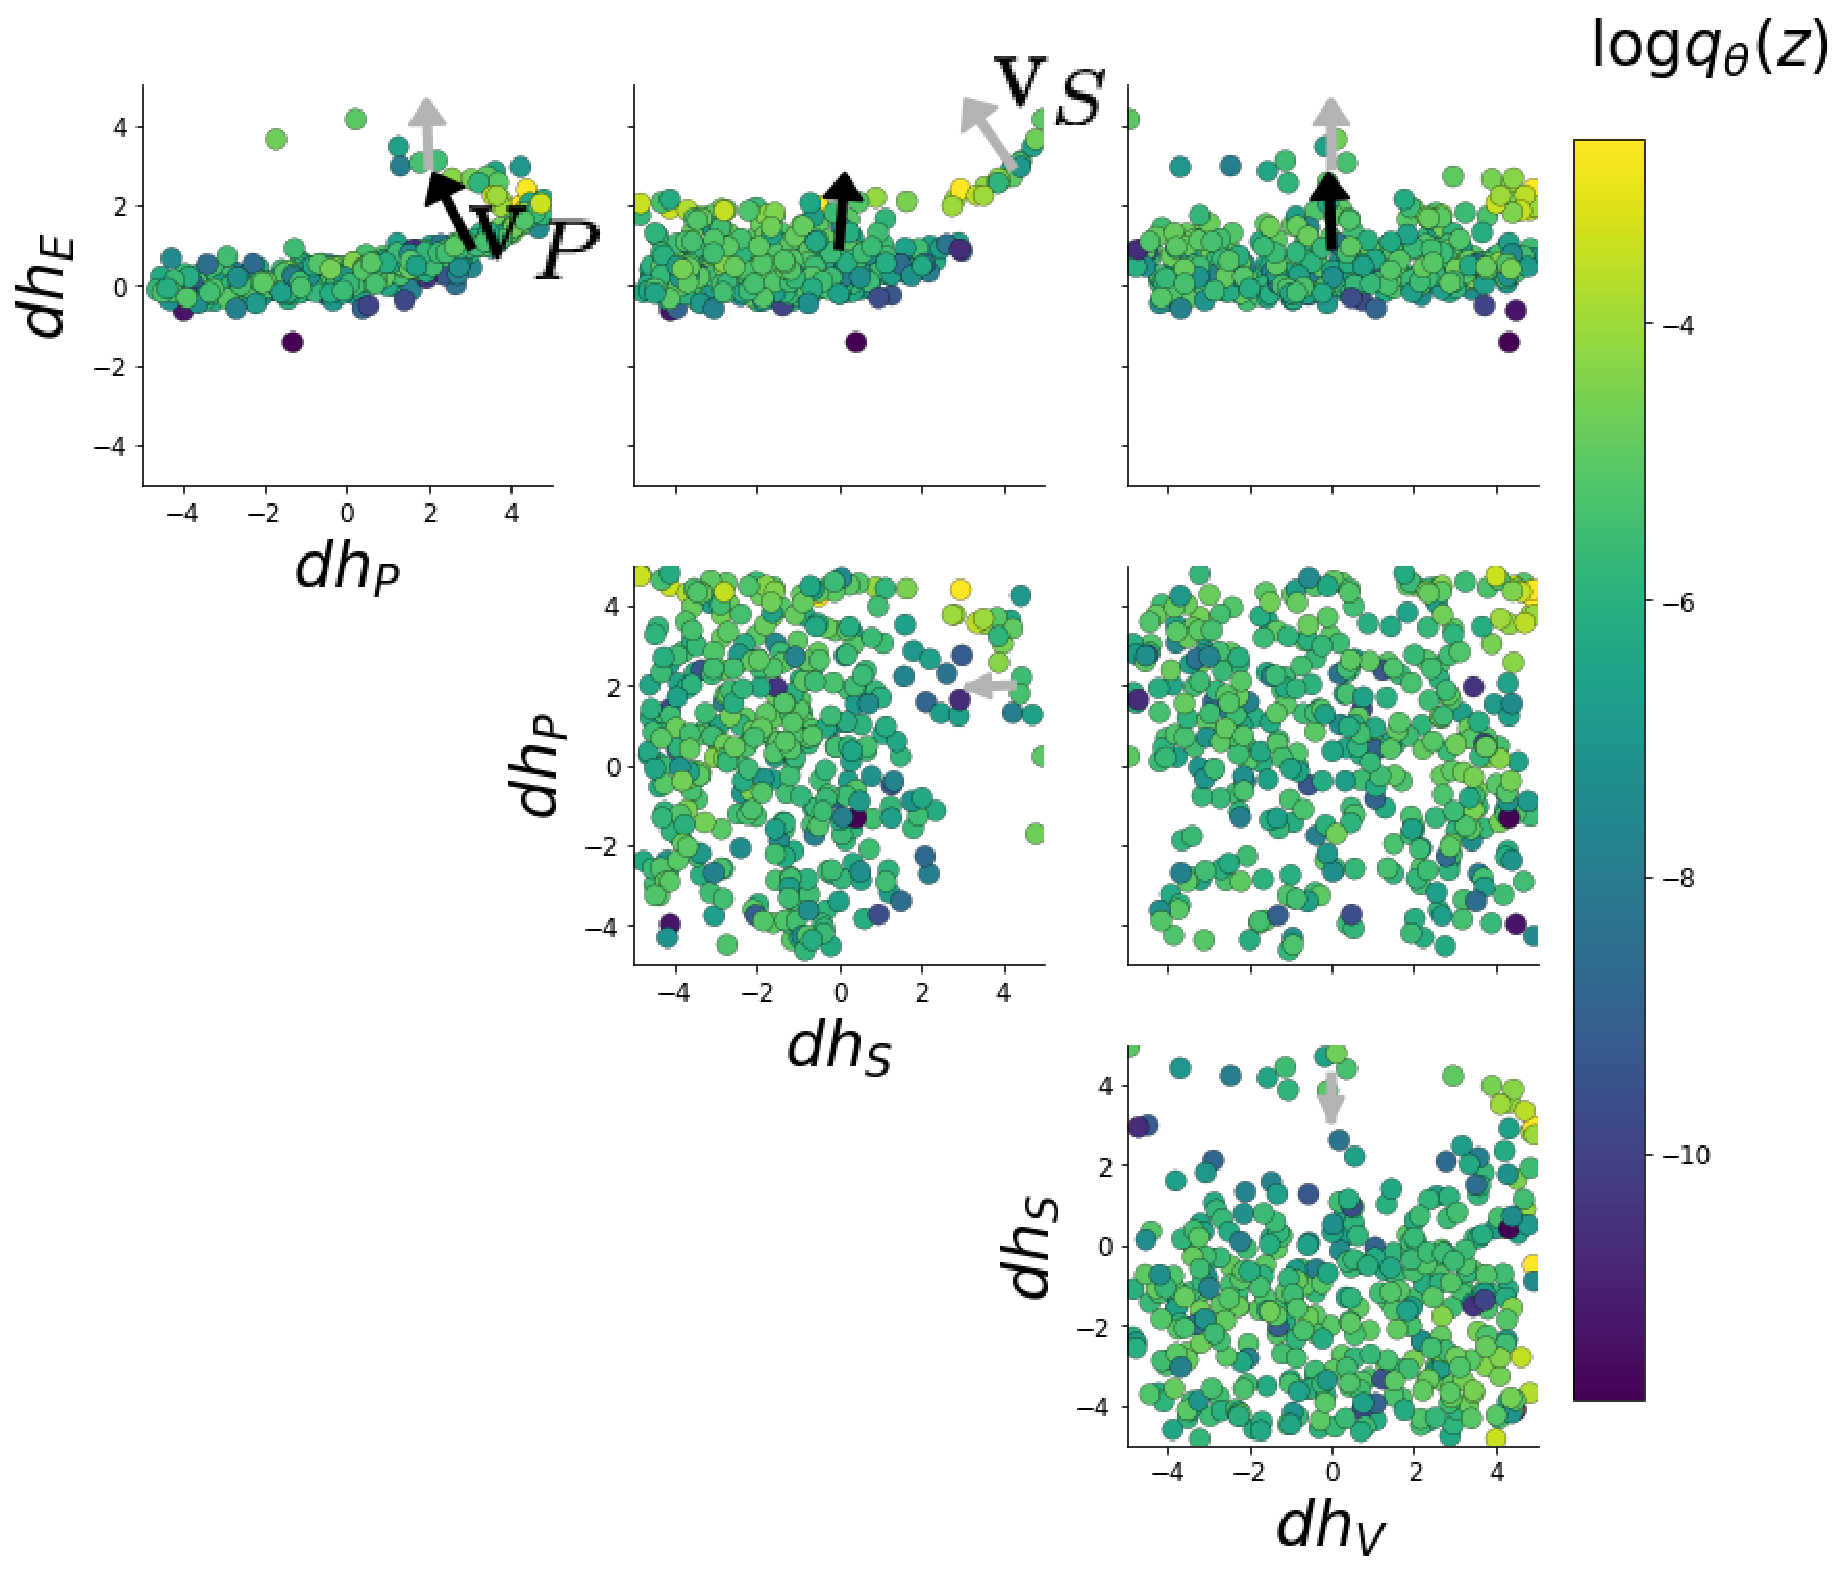
\includegraphics[scale=0.25]{figs/V1_drdh_EPI_E.pdf} 
\includegraphics[scale=0.25]{figs/V1_drdh_ABC_E.png} \\
\clearpage
$q_\theta(dh \mid \mathcal{B}(P,\sigma=0.25))$ \hspace{1.2in} $dh \sim ABC(P,\sigma_{ABC}=0.25)$. \\
\includegraphics[scale=0.25]{figs/V1_drdh_EPI_P.png} 
\includegraphics[scale=0.25]{figs/V1_drdh_ABC_P.png} \\
$q_\theta(dh \mid \mathcal{B}(S,\sigma=0.25))$ \hspace{1.2in} $dh \sim ABC(S,\sigma_{ABC}=0.25)$. \\
\includegraphics[scale=0.25]{figs/V1_drdh_EPI_S.png} 
\includegraphics[scale=0.25]{figs/V1_drdh_ABC_S.png} \\
$q_\theta(dh \mid \mathcal{B}(V,\sigma=0.25))$ \hspace{1.2in} $dh \sim ABC(V,\sigma_{ABC}=0.25)$. \\
\includegraphics[scale=0.25]{figs/V1_drdh_EPI_V.png} 
\includegraphics[scale=0.25]{figs/V1_drdh_ABC_V.png} \\
\end{center}

There are some subtle differences between the EPI and ABC distributions, but some difference is to be expected.
Rather than simply attributing these differences to imperfection of the EPI optimization routine, we consider the the effect of bias in $dx_\alpha$ from ABC (and lack thereof from EPI).

When $\epsilon > 0$ in ABC, the samples are \textit{not} from the posterior distribution.
For $\epsilon > 0$, the ``posterior" predictive means of ABC $\mathbb{E}_{ABC(\alpha, \sigma_{ABC})}\left[dx_\alpha \right]$ may be far from zero.
In Figure 3, we see that with ABC, there is an increasingly negative bias in $\mathbb{E}_{ABC(\alpha, \sigma_{ABC})}\left[dx_\alpha \right]$ for greater error tolerances across all neuron-types.  
Additionally with ABC, there is no precise control of the variance $\mathbb{E}_{ABC(\alpha, \sigma_{ABC})}\left[dx_\alpha^2 \right]$, which may be undesireable.

In contrast, the first and second moments of $dx_\alpha$ are controlled to a specified degree of accuracy (Figure 4).
The variances of each distribution of $dx_\alpha$ are close to their target value $0.25^2 = 0.0625$ (see variances next to histograms of Figure 4). 
The regions of the ABC pairplots which have $|dx_\alpha| \approx 0.5$ are far less probable in the EPI distributions (by design), and can account for most mismatch observed.
As a note, there is a discontinuity in Figure 2, $EPI(E, \sigma=0.25)$ in the $dh_E$-$dh_S$ plane.
I'd like to see if I can run the optimization for more random seeds so that we obtain a more connected distribution.

\begin{center}
\textbf{Figure 3: Biased ABC} \\
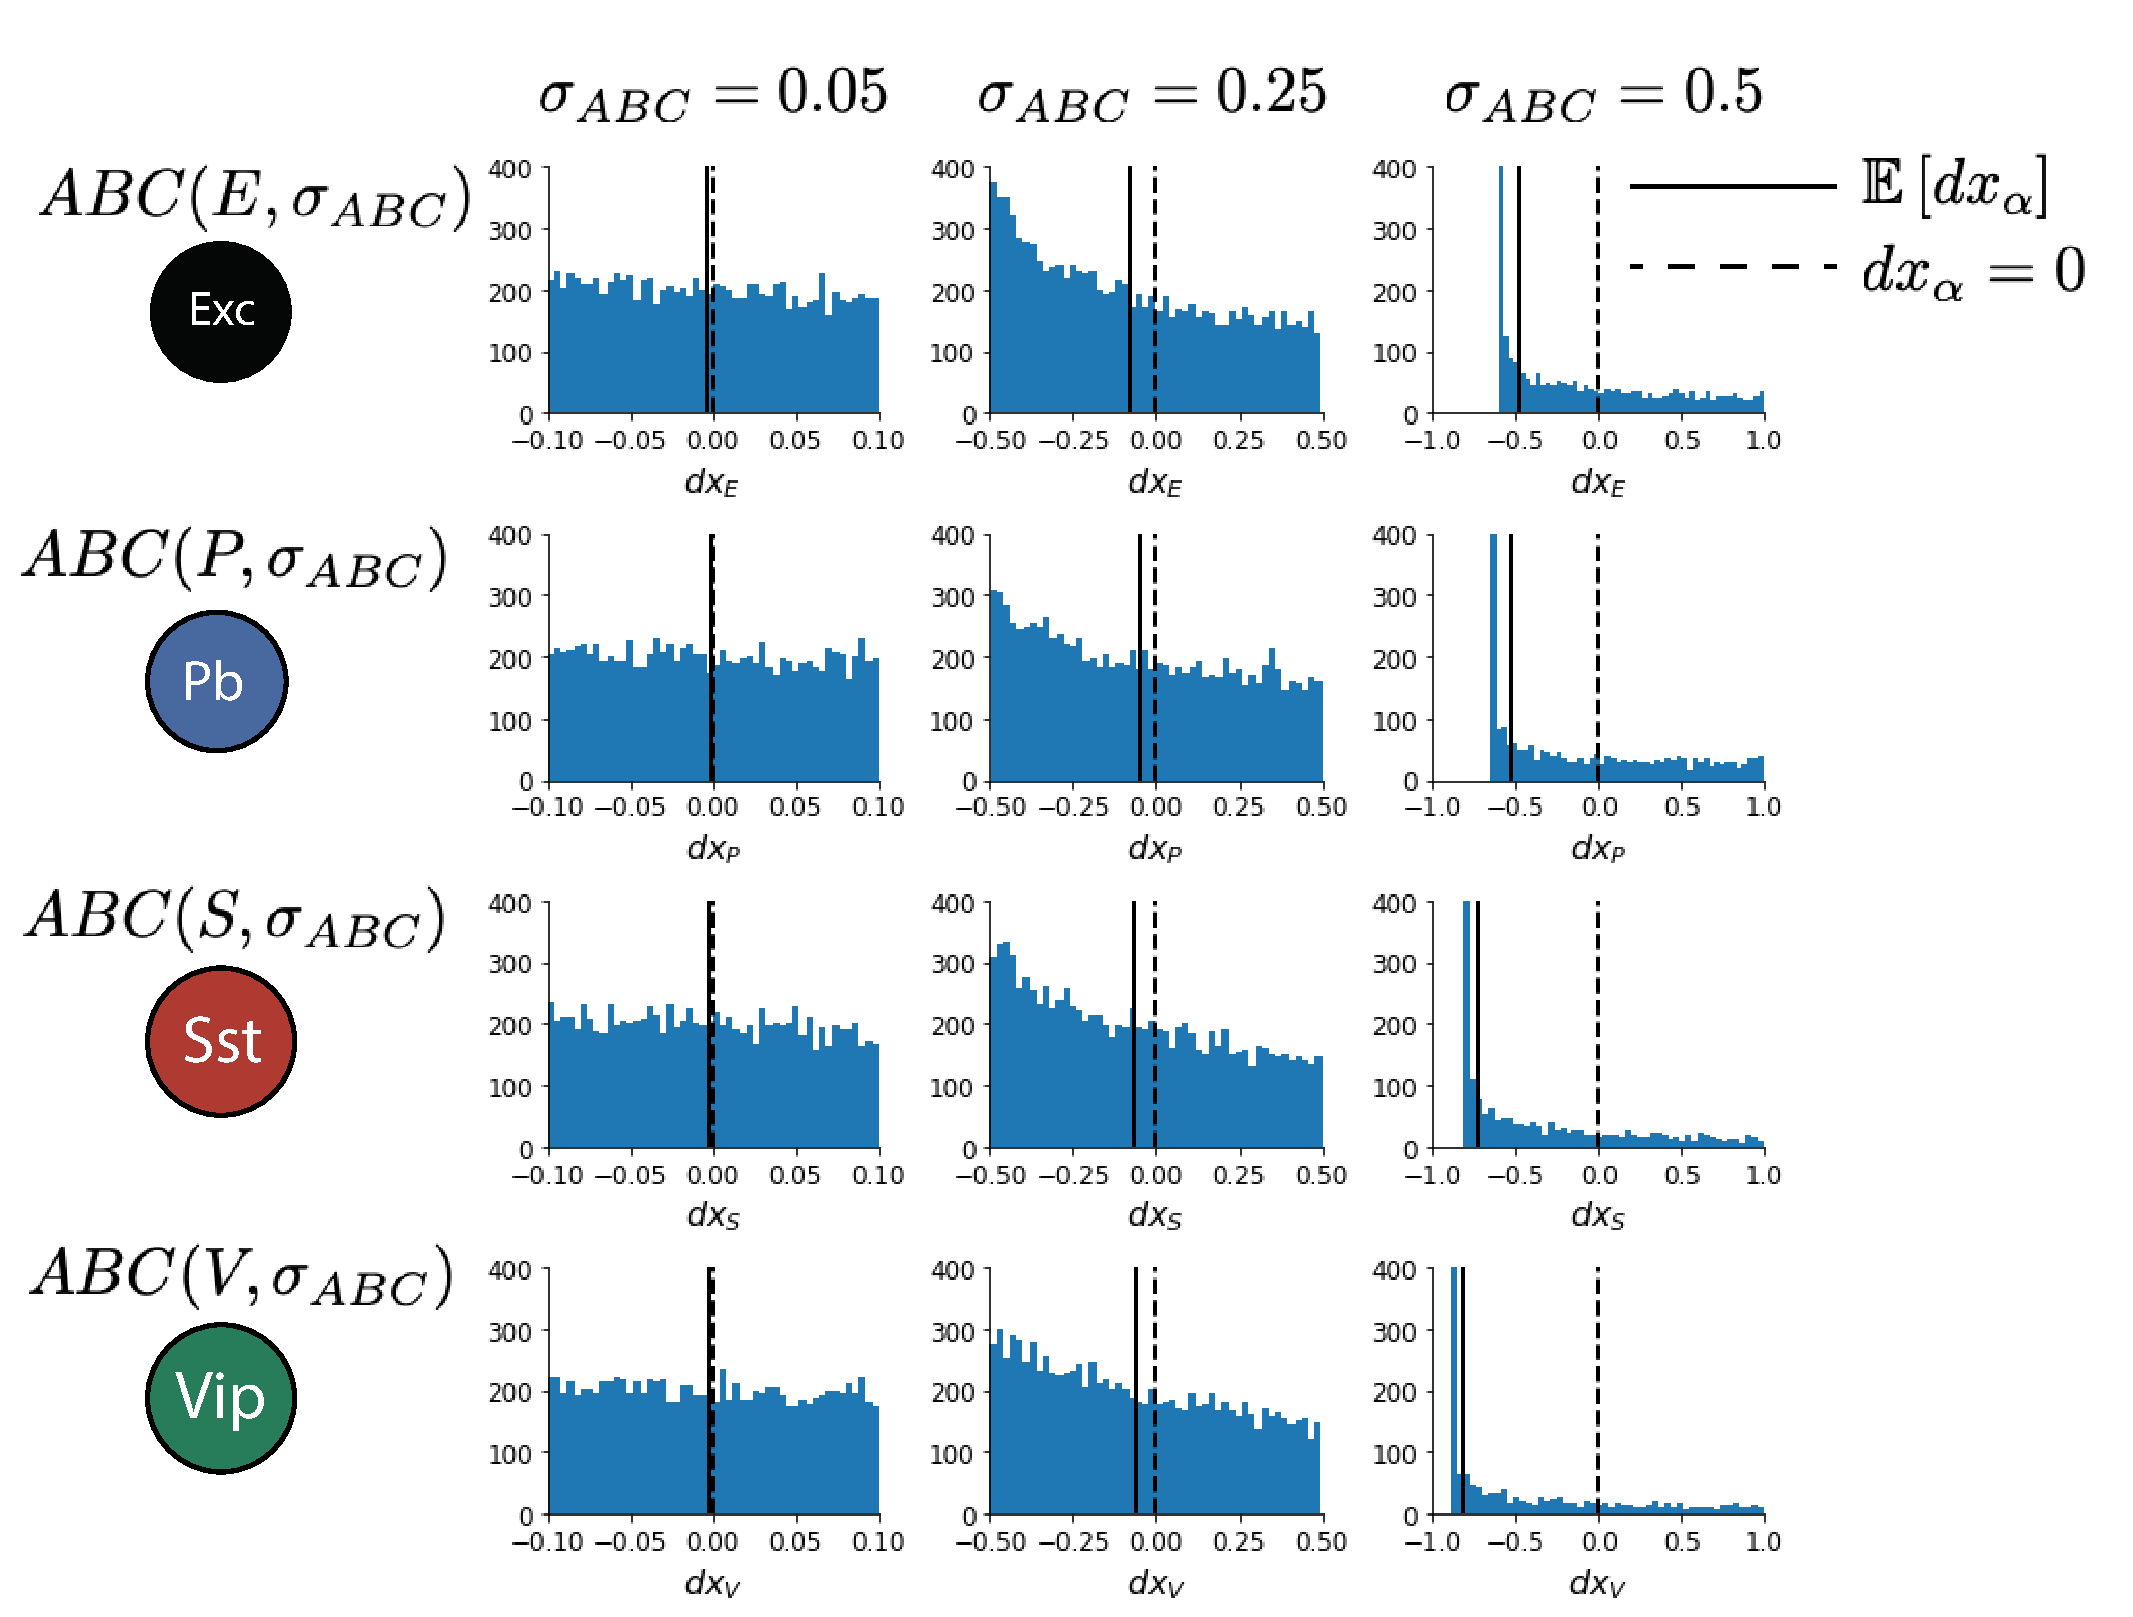
\includegraphics[scale=0.4]{figs/V1_ABC_Tx.pdf}
\end{center}

\clearpage

\begin{center}
\textbf{Figure 4: Unbiased EPI} \\
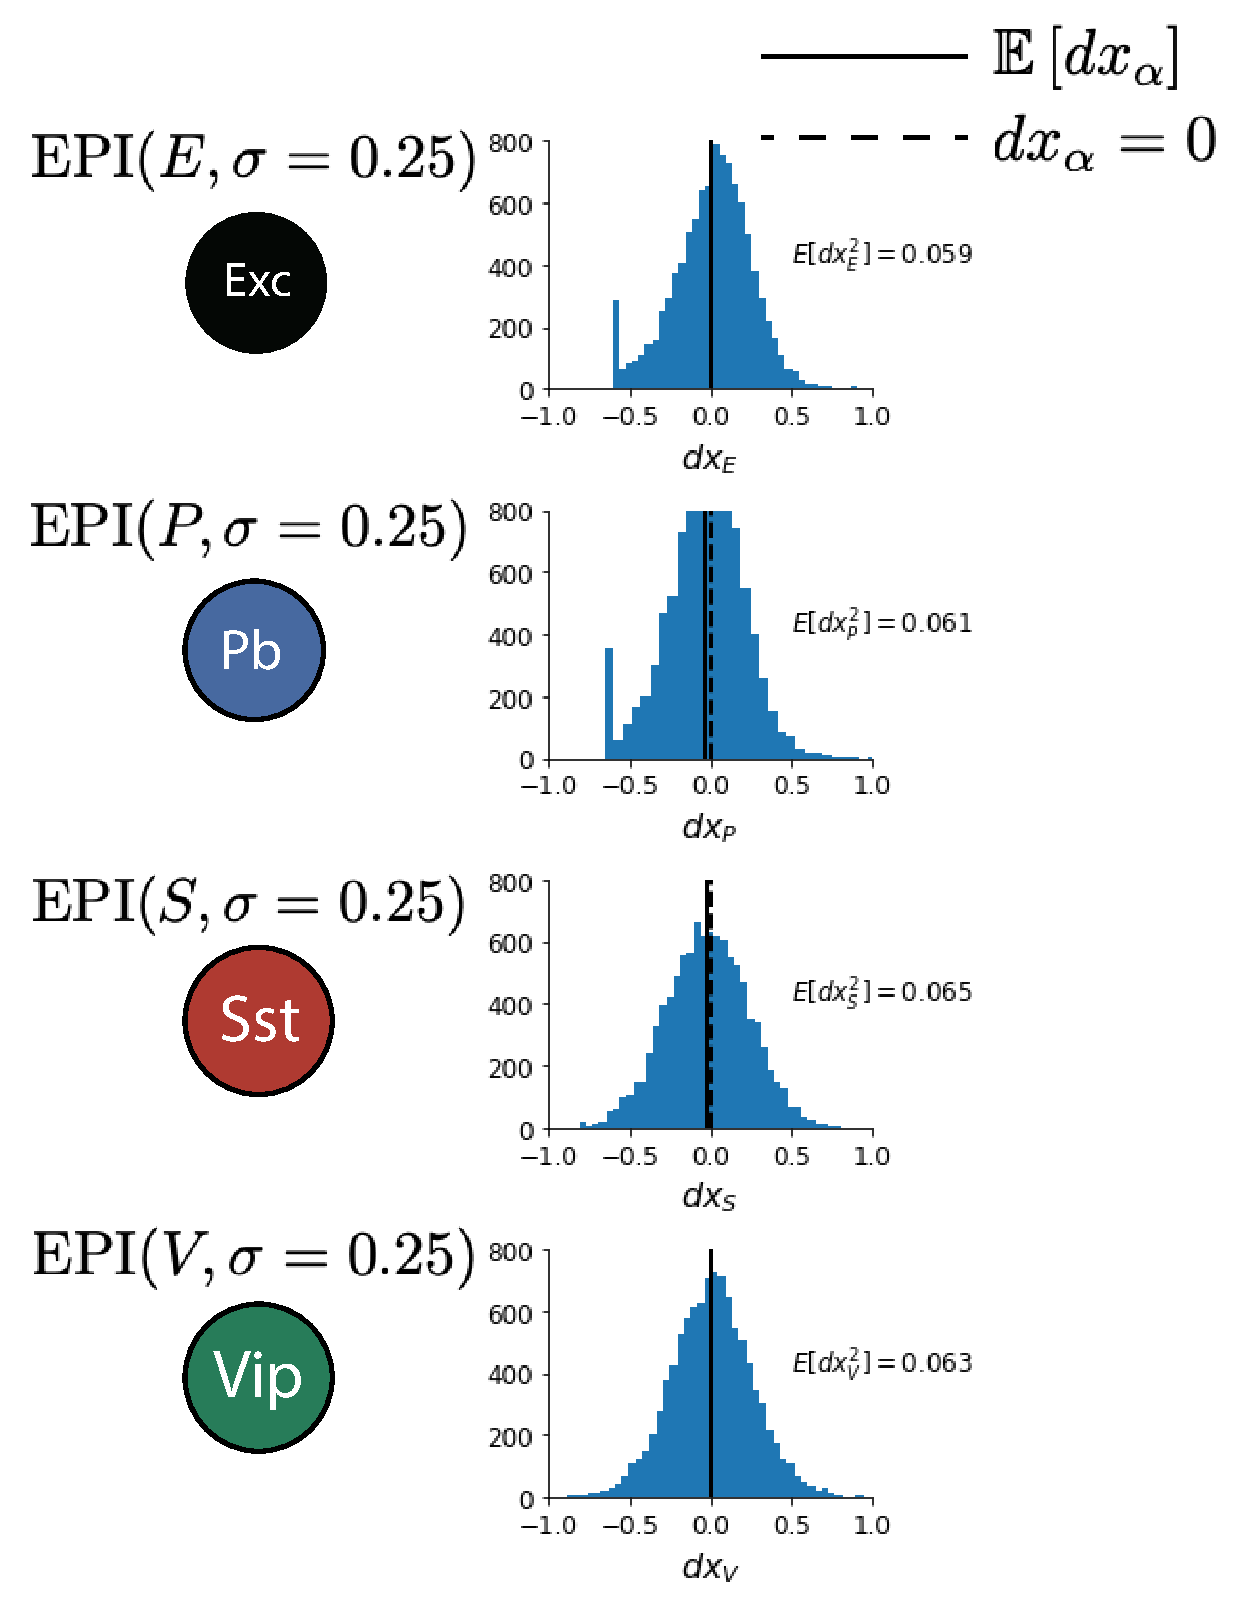
\includegraphics[scale=0.4]{figs/V1_EPI_Tx.pdf}
\end{center}

\section{EPI-enabled analyses}
\subsection{Dimensions of sensitivity}
Each arrow in the EPI distributions (Fig. 2, left) points in the direction of maximal sensitivity indicated by the hessian $\partial^2 \log q_\theta(dh) / \partial dh \partial dh^\top$ evaluated at the $dh$ at the base of the arrow.
These patterns of input elicit a greater $dx_\alpha^2$ than (at least) 98.8\% of random stimulation patterns.
Each sensitivity vector is representative of a different stabilization mechanism.

\subsection{Confiriming distinct mechanisms of stabilization}
The sensitivity arrows on the EPI distribution for E-population stability (Fig. 2, top, left) indicate two distinct stability mechanisms for increased $dh_E$.
In one case, $dh_P$ must increase along with increased $dh_E$ (Fig. 2, top, left black arrow $v_P$).
In the other case, $dh_S$ must increase along with increased $dh_E$ (Fig. 2, top, left gray arrow $v_S$).
These inferred distributions and sensitivity vectors $v_P$ and $v_S$ motivate the following hypothesis:

H: If the P- and S-populations are inactivated, the only E-stabilization mechanism with increasing $dh_E$ will be that of the other population (S- or P-population, respectively) .

We can test this hypothesis with EPI, since it is optimized to identify the distribution of all inputs resulting in E-population stability.
We ran EPI with the same emergent property as Eq 2 ($\alpha=E$, $\sigma=0.25$) for two different inactivation scenarios.
In the P-inactivated case, we changed the baseline input to $b =b_{\not P} \triangleq \left[ 1, -5, 1 ,1.25 \right]^\top$, and to $b =b_{\not S} \triangleq \left[ 1, 1, -5 ,1.25 \right]^\top$ in the S-inactivated case.
To test for the existence of stabilization mechanisms corresponding to $v_P$ and $v_S$, we measured the most-sensitive dimension of the Hessian at all points in the inferred distribution.  
We declare that the P- or S-inactivated circuit lacks a stability mechanism, if no sensitivity vectors throughout the distribution are aligned with the corresponding sensitivity vector.

\begin{center}
\textbf{Figure 5}: Stability mechanisms of inactivated circuits.
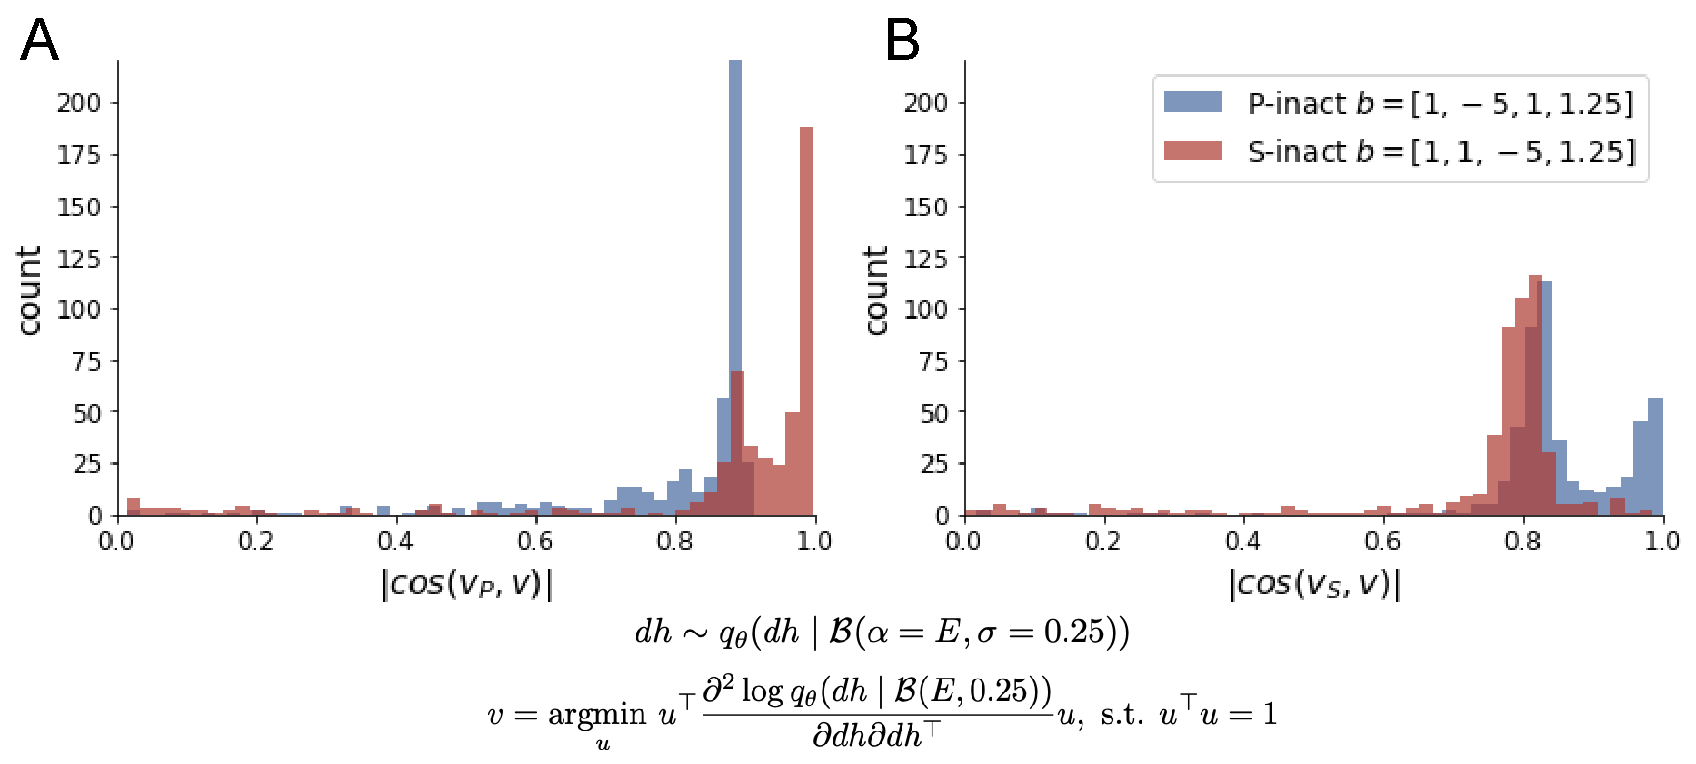
\includegraphics[scale=.5]{figs/cos_dists.pdf}
\end{center}

Confirming our hypothesis, we found that only the $v_S$ stability mechanism is present in the P-inactivated circuit (Figure 5A), and that only the $v_P$ stability mechanism is present in the S-inactivated circuit (Figure 5B).
As expected, the samples of the inferred distributions aligned with the stability mechanism correspond to the sloped regions orthogonal to $v_S$ and $v_P$ (Figure 6).

\clearpage

\begin{center}
\textbf{Figure 6}: Inactivated circuit stability distributions.
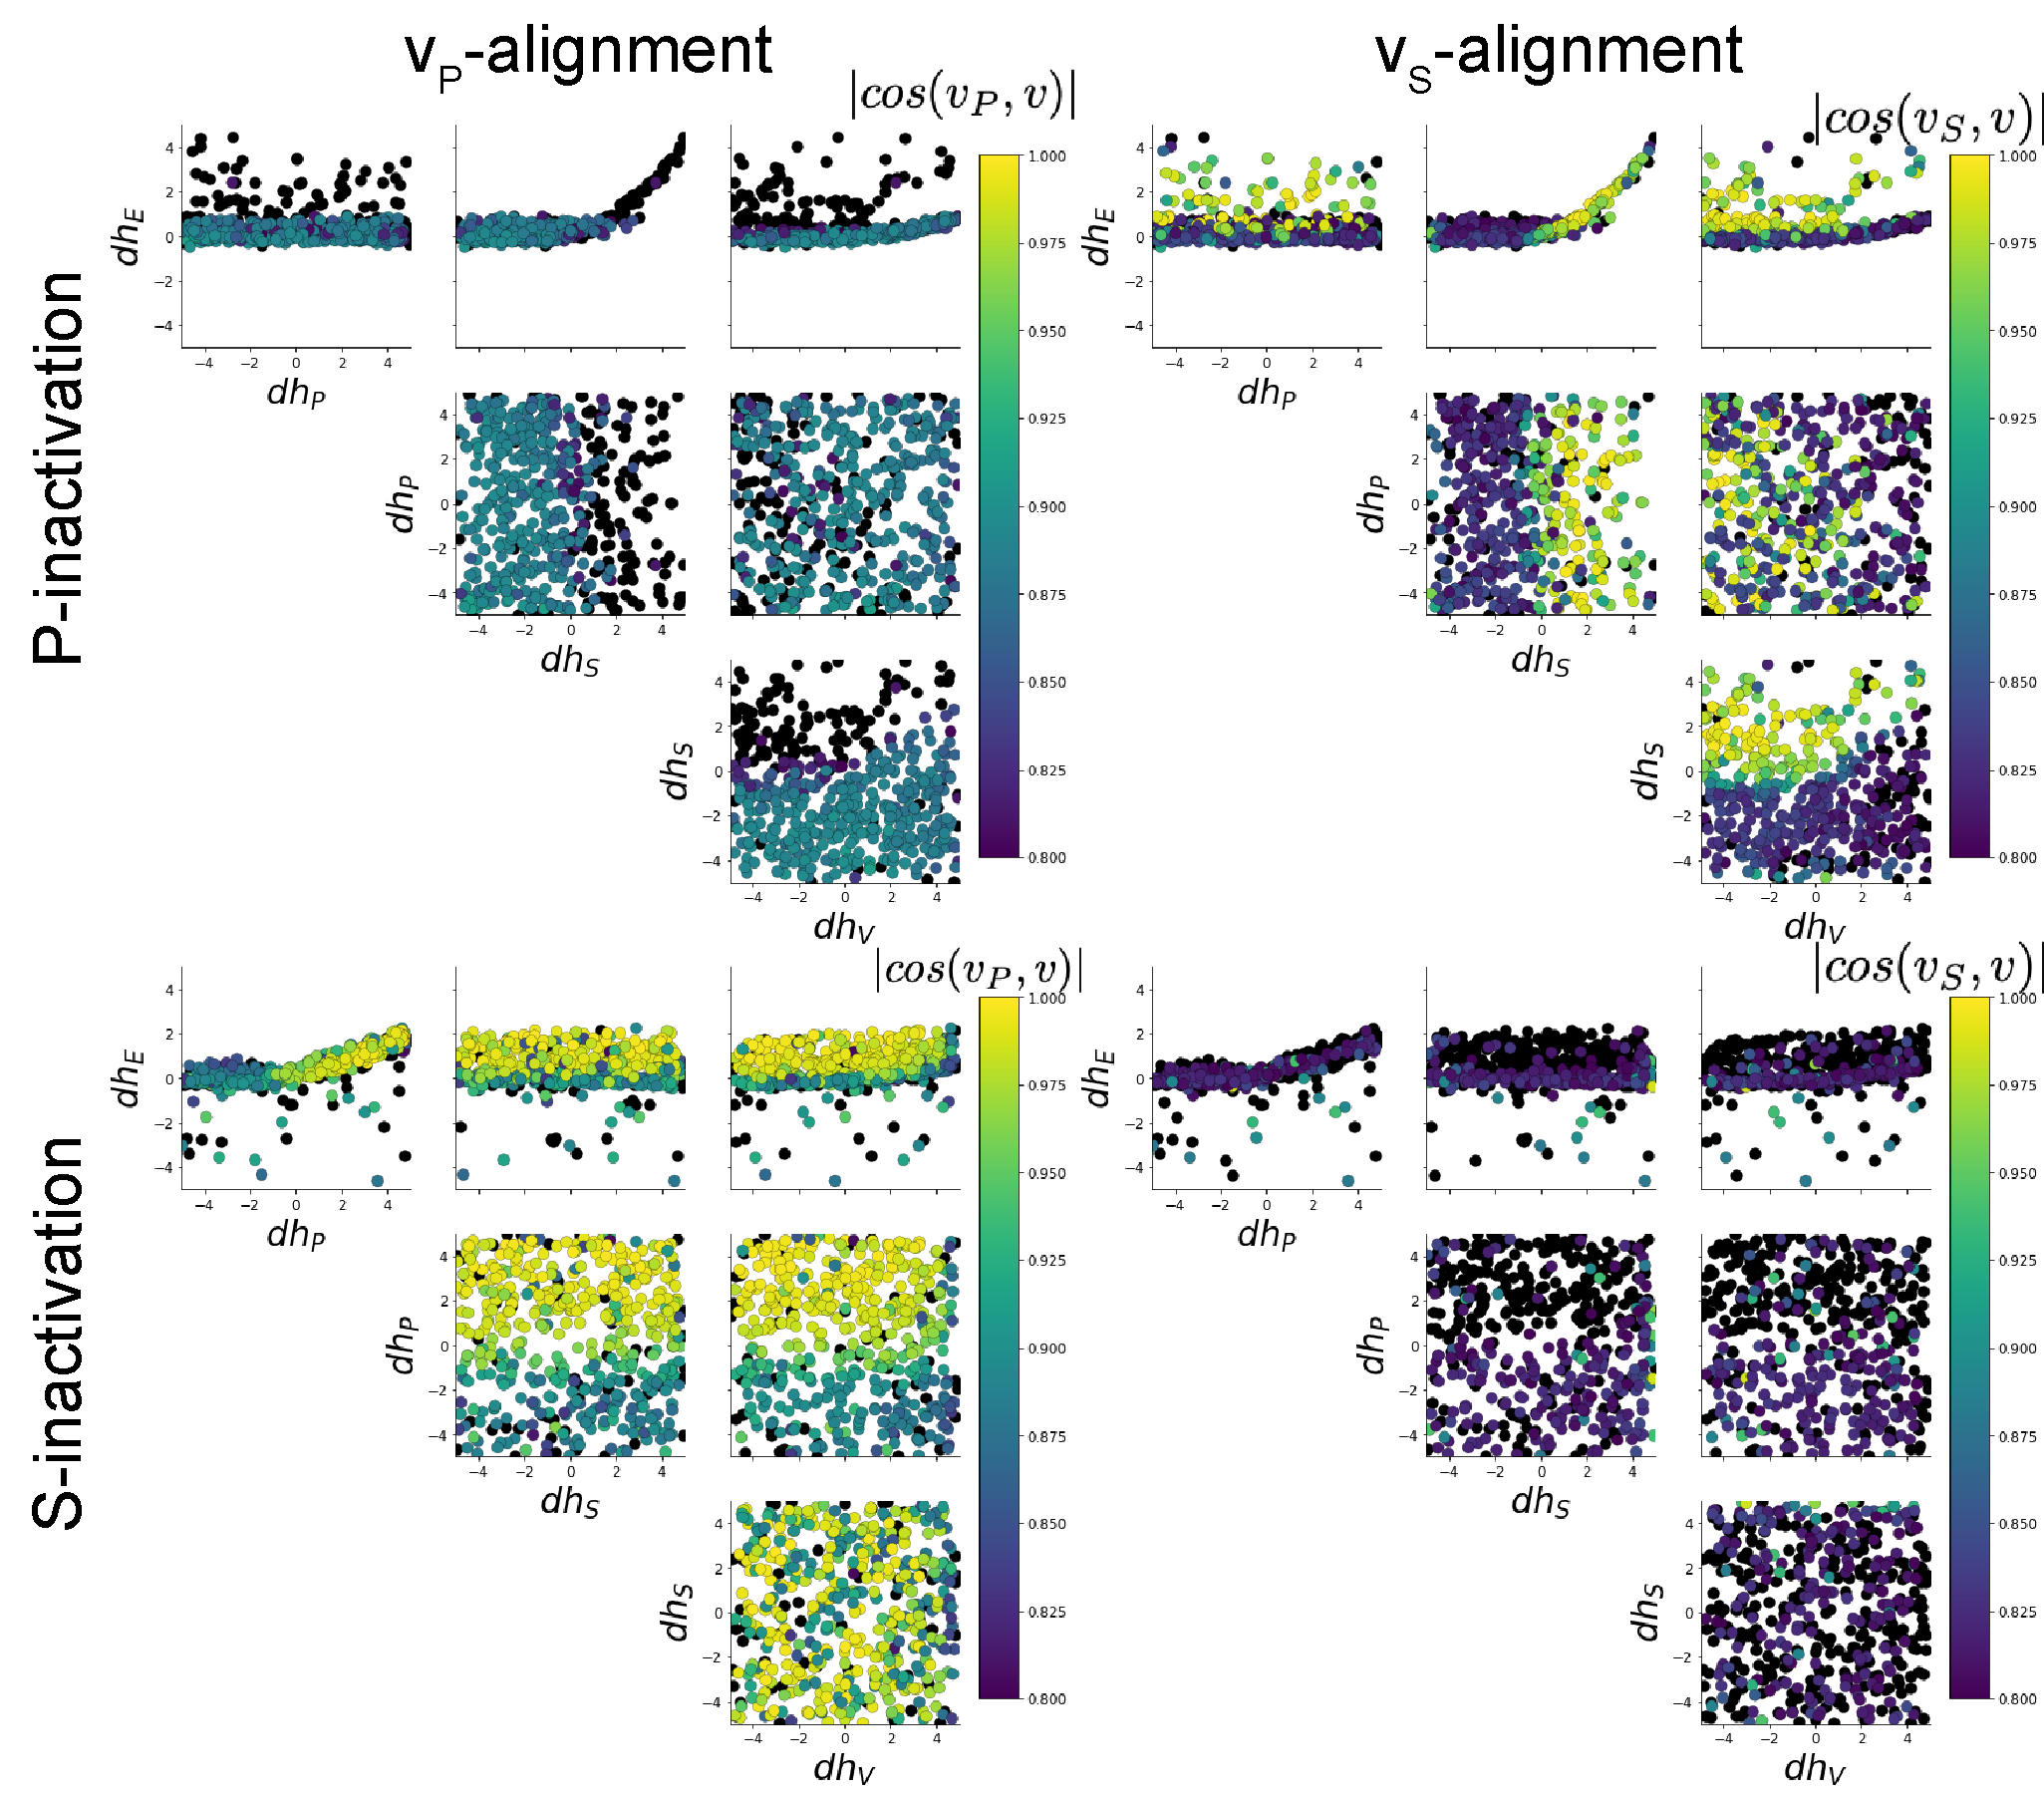
\includegraphics[scale=.4]{figs/EPI_inactivation.pdf}
\end{center}

\section{Summary}
We have improved on our previous EPI analysis of V1 in the following ways:
\begin{enumerate}
\item We utilize a novel ability of EPI (Hessian evaluation).
\item Our scientific conclusion is about mechanisms of stability rather than high-level characteristics of responses.
\item We have validation of structure via ABC.
\item We characterize the issue of bias in ABC (and lack thereof in EPI).
\item The emergent property of ``neuron-type stabilization" follows the ethos of the definition of emergent property better than ``neuron-type population rate increase of $y$".
\end{enumerate}

I recommend substituting this work for section 3.3 in the bioRxiv manuscript. I'd be happy to write up a draft of such a section.


%\section{Isolated modulation paths using EPI}
%Let's say we want to find a stimulation pattern that changes the $\alpha$-population steady-state response $dx_\alpha$ as much as possible while keeping the rest the same.
%One can not simply stimulate the $\alpha$-population, since one must take into account the effects of the recurrent connectivity.
%Furthermore, such an input pattern producing isolated modulation may change nonlinearly.
%
%Beginning at $dh = \textbf{0}$, we seek a sequence of differential inputs that will increasingly change $dx_\alpha$, while maintaining $dx_\beta$, $\beta \in \{E, P, S, V\} \setminus	\{\alpha\}$.
%At each step in the path of inputs, the direction is selected to maximize change in $dx_\alpha$ and minimize change in $dx_{\beta \neq \alpha}$.
%These input selections can be guided by the EPI distributions $q_\theta(dh \mid \mathcal{B}(\alpha, 0.2))$ that result in the modulation of the $\alpha$ population within a given range.
%
%We leverage the availability of a functional representation of $\log q_\theta(dh \mid \mathcal{B}(\alpha, 0.2))$ to calculate the the hessians of the EPI distributions at each step of $dh$ in the path
%\begin{equation}
%\text{Hess}_\alpha(dh) = \frac{\partial^2 \log q_\theta(dh \mid \mathcal{B}(\alpha, 0.2))}{\partial dh \partial dh^\top}.
%\end{equation}
%
% We select the optimal direction of isolated modulation as vector v, which points in the maximally decreasing dimensions of $\log q_\theta(dh \mid \mathcal{B}(\alpha, 0.2))$, and minimally decreasing dimensions of $\log q_\theta(dh \mid \mathcal{B}(\beta, 0.2))$, $\beta \neq \alpha$:
% \begin{equation}
% v_\alpha^*(dh) = \argmin_v v^\top \text{Hess}_\alpha(dh) v - \sum_{\beta \neq \alpha} v^\top \text{Hess}_\beta(dh) v,
% \end{equation}
%  where $v\top v$ = 1.  $v_\alpha(dh)$ is obtained via an eigendecomposition:
%  \begin{equation}
%  v_\alpha^*(dh) = \argmin_v v^\top M_\alpha(dh) v
% \end{equation}
% \begin{equation}
%M_\alpha(dh) = \text{Hess}_\alpha(dh) - \sum_{\beta \neq \alpha} \text{Hess}_\beta(dh).
% \end{equation}
% The solution is the eigenvector with smallest eigenvalue of $M_\alpha(dh)$.
% 
% 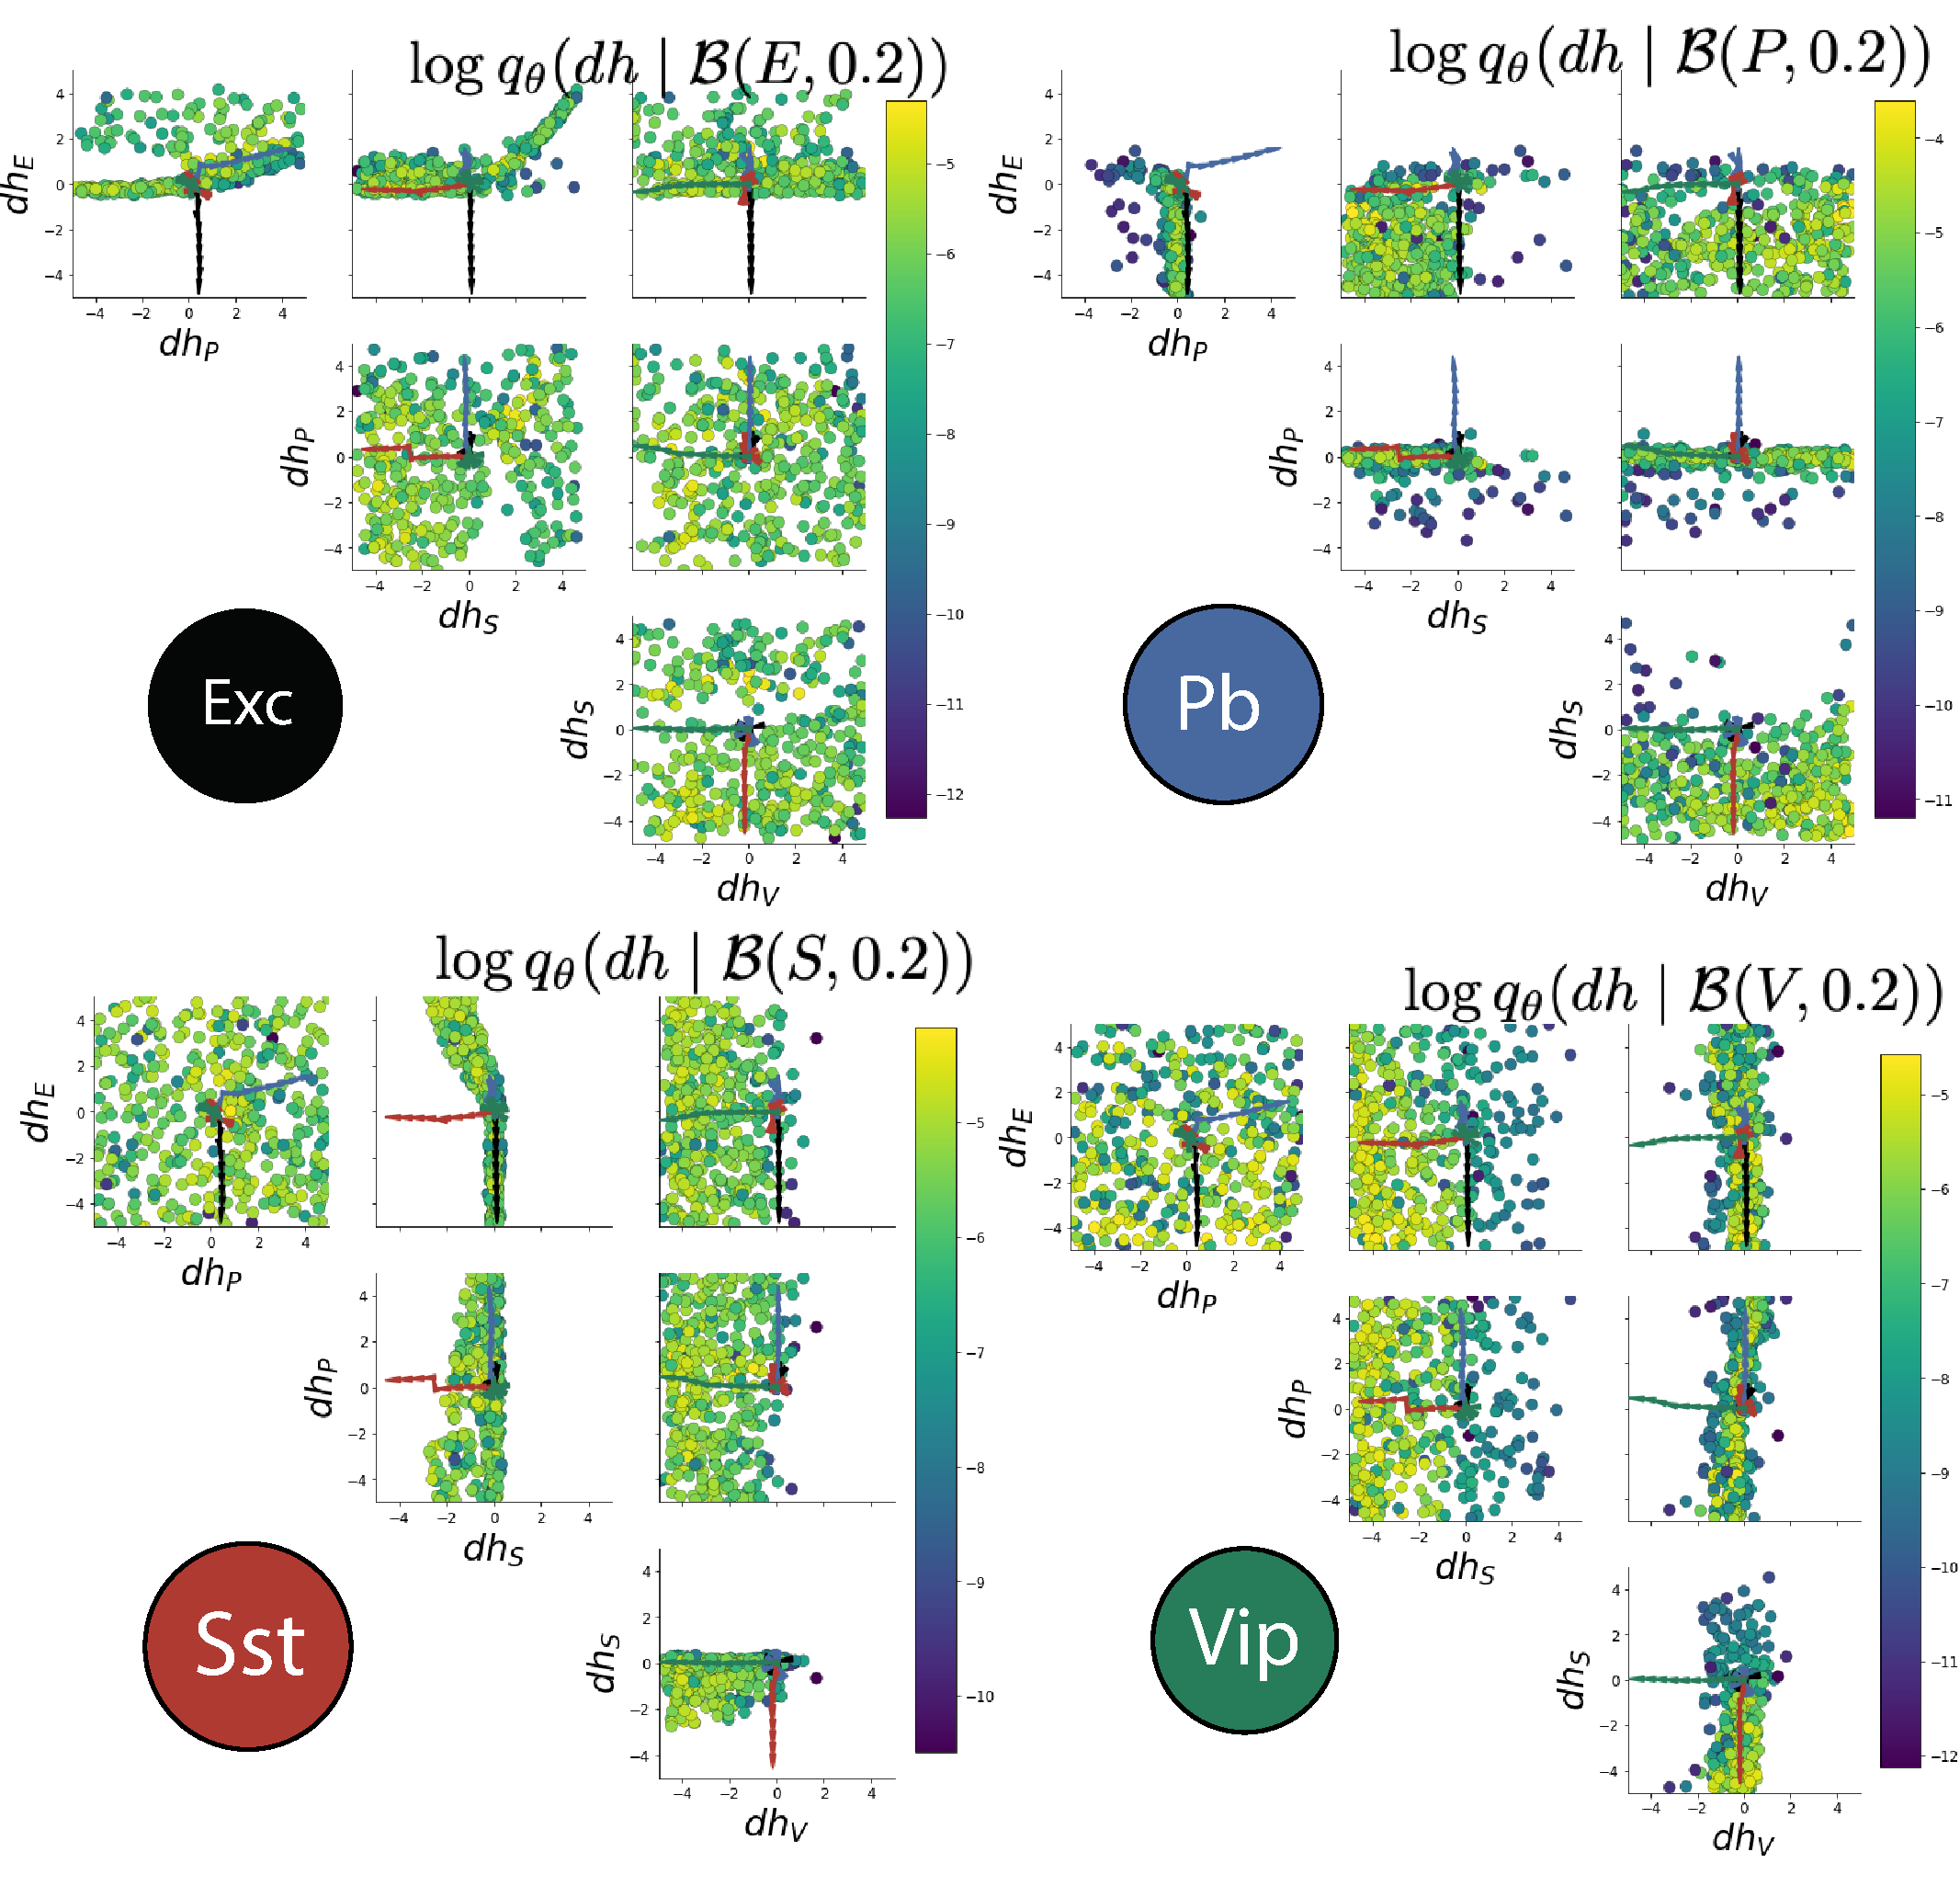
\includegraphics[scale=0.4]{figs/hess_paths.pdf}
% 
 


\bibliography{epi}
\bibliographystyle{unsrt}

\end{document}

